\documentclass[11pt,a4paper]{article}
\usepackage[margin=1in]{geometry}
\usepackage{graphicx}
\usepackage{booktabs}
\usepackage{hyperref}
\usepackage{amsmath,amssymb}
\usepackage{xcolor}
\usepackage{enumitem}
\usepackage{caption}
\usepackage{subcaption}
\usepackage{float}
\usepackage{tabularx}
\usepackage{multirow}
\usepackage[T1]{fontenc}

\hypersetup{colorlinks=true,linkcolor=blue!60!black,citecolor=green!50!black,urlcolor=blue!60!black}

\setlength{\parskip}{0.4em}
\setlength{\parindent}{0em}

\newcommand{\A}{\mathbf{A}}

\title{\textbf{DAGFormer: Learned Computation Graphs\\for Transformers}\\[0.5em]
\large Progress Report --- March 2026}
\author{}
\date{}

\begin{document}
\maketitle
\thispagestyle{empty}

\begin{abstract}
This report summarizes our experiments on learning input-dependent computation graphs (DAGs) for transformer language models. We cover two lines of work: \textbf{midtraining} on a pretrained OLMo-1B (Section~2), and \textbf{pretraining from scratch} with a 300M model (Section~3). Midtraining failed because $\A=\mathbf{1}$ (dense connectivity) is a flat optimum for pretrained weights. Pretraining from scratch shows that self-embed predictors \emph{can} learn meaningful sparse topologies (mean $\A \approx 0.42$), but a 3.5$\times$ throughput overhead makes direct comparison unfair. We present five new strategies currently under evaluation and propose additional recipes for discussion.
\end{abstract}

%═══════════════════════════════════════════════════════════
\section{Introduction}
%═══════════════════════════════════════════════════════════

Standard transformers use a fixed sequential computation graph: layer $0 \to 1 \to \cdots \to L$. Every input sees the same wiring regardless of content. \textbf{DAGFormer} replaces this with a learned, input-dependent directed acyclic graph (DAG) that controls which attention heads feed into which other heads.

The core modification: each attention head $j$ in layer $l$ receives a \emph{gated combination} of prior heads' outputs:
\[
\text{input}_j = \text{embedding} + \sum_{l' < l} \text{mlp}_{l'} + \sum_{i:\,\text{layer}(i)<l} \A[i,j] \cdot \text{head\_output}[i]
\]
where $\A \in [0,1]^{N \times N}$ ($N = \text{layers} \times \text{heads}$) is block-upper-triangular. When $\A[i,j]=1$ for all valid pairs, this reduces to the standard residual stream.

\paragraph{Oracle motivation.} An oracle search (500 gradient steps per 1024-token window, directly optimizing $\A$) reduced NLL from 2.58 to 0.12 on OLMo-1B (median across 50 windows, 100\% improved). This demonstrates enormous headroom but is too slow for practical use. DAGFormer aims to \emph{amortize} this search into a learned predictor.

\paragraph{Architecture.} The predictor maps input context to $\A$ via: context $\to$ encoder $\to$ MLP $\to$ low-rank $Z = UV^\top + b$ $\to$ mask $\to$ Gumbel-Sigmoid $\to$ cascading gate $\to$ $\A$. Training is end-to-end: NLL gradients flow through the modified OLMo forward back to the predictor. See \texttt{structure\_predictor.html} for the full interactive architecture diagram.


%═══════════════════════════════════════════════════════════
\section{Midtraining on Pretrained OLMo-1B}
%═══════════════════════════════════════════════════════════

Our first approach: keep the pretrained OLMo-1B and learn topology on top of it. We explored \textbf{Phase~1} (frozen OLMo, only predictor trains) and \textbf{Phase~2} (unfrozen OLMo, joint training). Both failed.

%───────────────────────────────────────────────────────────
\subsection{Phase 1: Frozen OLMo --- $\A=1$ Is a Flat Optimum}

With OLMo frozen, any deviation from $\A=\mathbf{1}$ hurts. We tested multiple \texttt{init\_logit} values controlling how far from dense the predictor starts:

\begin{figure}[H]
\centering
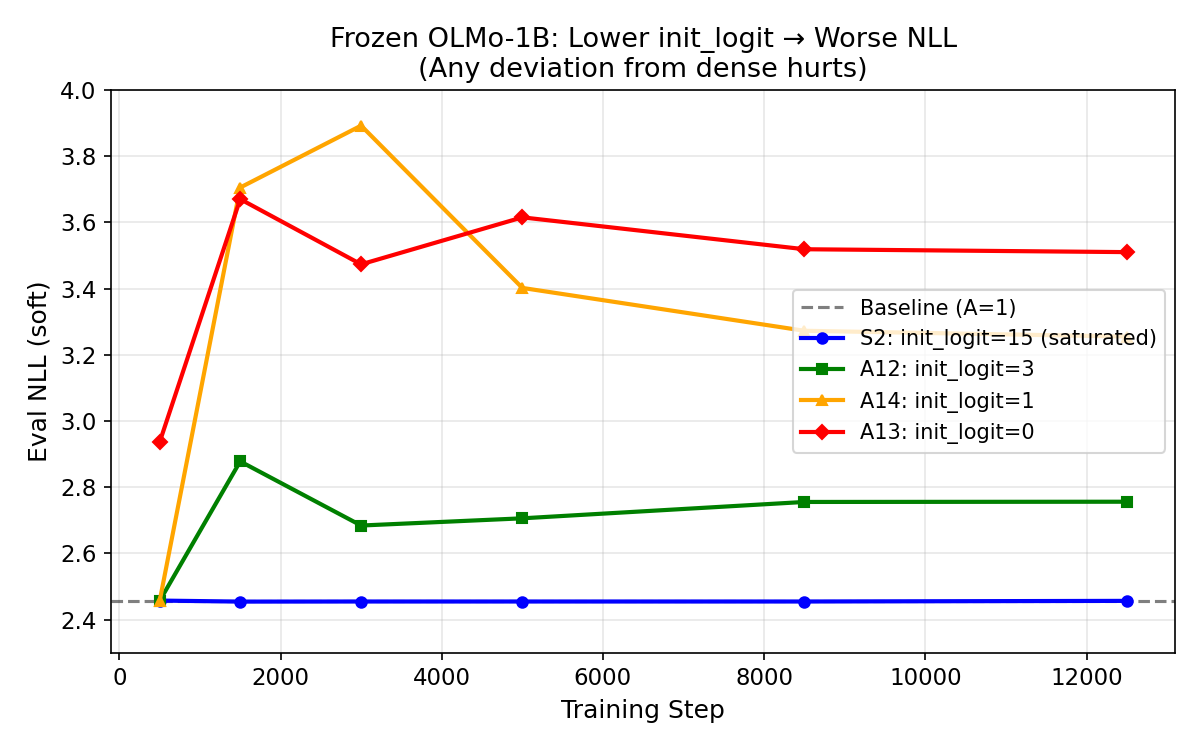
\includegraphics[width=0.82\textwidth]{figures/fig1_init_logit_ablation.png}
\caption{Frozen OLMo-1B: lower \texttt{init\_logit} $\to$ further from dense $\to$ worse NLL. S2 (\texttt{init\_logit}=15) stays at baseline but has saturated sigmoid (no gradient). A12/A13/A14 have gradient flow but converge to fixed topologies \emph{worse} than dense.}
\label{fig:init_logit}
\end{figure}

To understand \emph{why} $\A=\mathbf{1}$ is optimal, we computed $\partial\mathcal{L}/\partial\A$ at $\A=\mathbf{1}$ across 50 eval windows:

\begin{figure}[H]
\centering
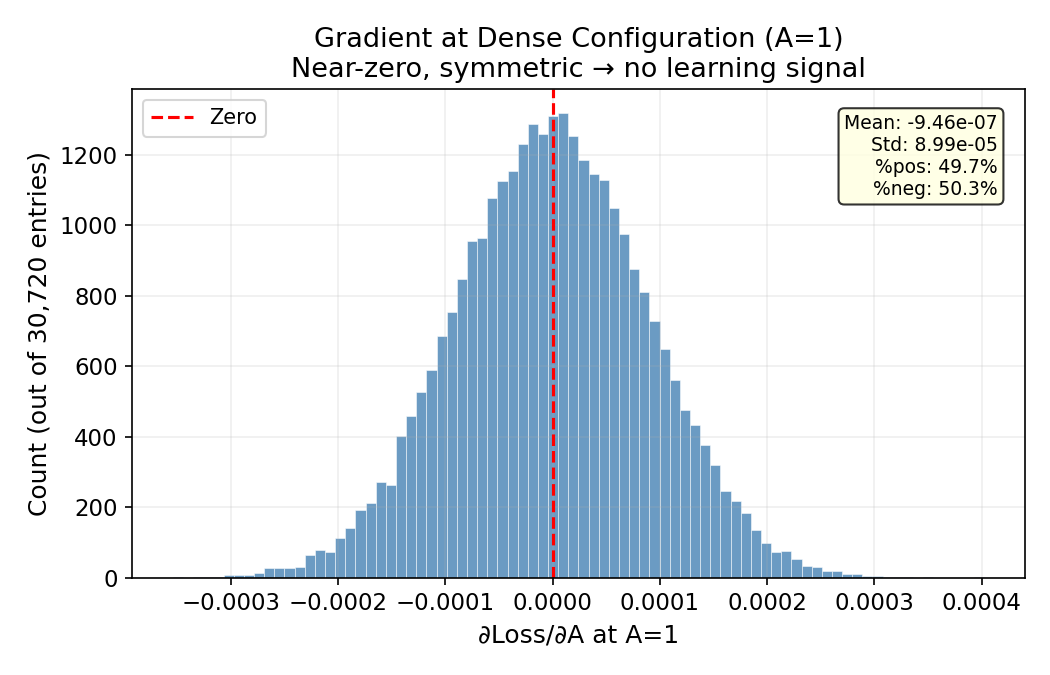
\includegraphics[width=0.72\textwidth]{figures/fig2_gradient_at_A1.png}
\caption{Gradient at $\A=\mathbf{1}$: symmetric around zero (49.7\% positive, 50.3\% negative, mean $\approx 10^{-6}$, std $\approx 9 \times 10^{-5}$). No consistent direction exists. Pretrained weights make $\A=\mathbf{1}$ a flat plateau.}
\label{fig:gradient}
\end{figure}

%───────────────────────────────────────────────────────────
\subsection{Phase 2: Unfrozen OLMo --- The LR Dilemma}

Unfreezing OLMo allows the model to adapt to non-dense topologies. We ran 10 experiments varying OLMo LR, predictor LR, temperature schedule, initialization, and sparsity pressure.

\begin{figure}[H]
\centering
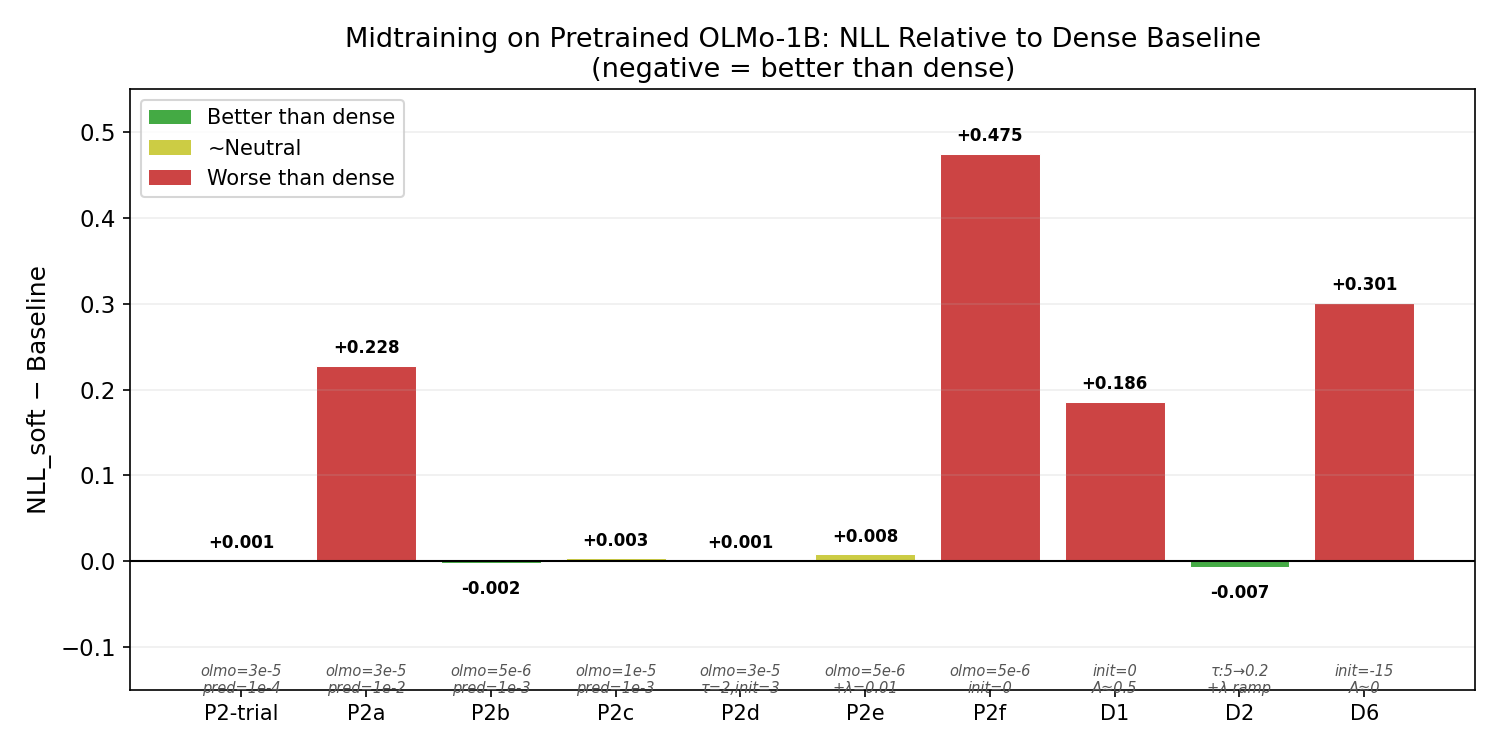
\includegraphics[width=0.95\textwidth]{figures/fig3_midtrain_all_results.png}
\caption{NLL relative to dense baseline for all 10 midtraining experiments. Only P2b ($-0.002$) and D2 ($-0.007$) show improvement; both remain near-dense (mean $\A > 0.97$). Most experiments are substantially worse.}
\label{fig:midtrain_all}
\end{figure}

The core dilemma:
\begin{itemize}[nosep]
\item \textbf{High OLMo LR}: OLMo quickly adapts to dense via CPT. The predictor has no incentive to deviate from $\A \approx 1$.
\item \textbf{Low OLMo LR}: OLMo cannot adapt to non-dense topologies. Any deviation from $\A=\mathbf{1}$ destroys information.
\item \textbf{High predictor LR}: Topology collapses to random (P2a: mean $\A=0.5$, NLL $+0.23$).
\item \textbf{Starting sparse} (D1, D6): OLMo is damaged by missing connections it relies on.
\end{itemize}

\begin{figure}[H]
\centering
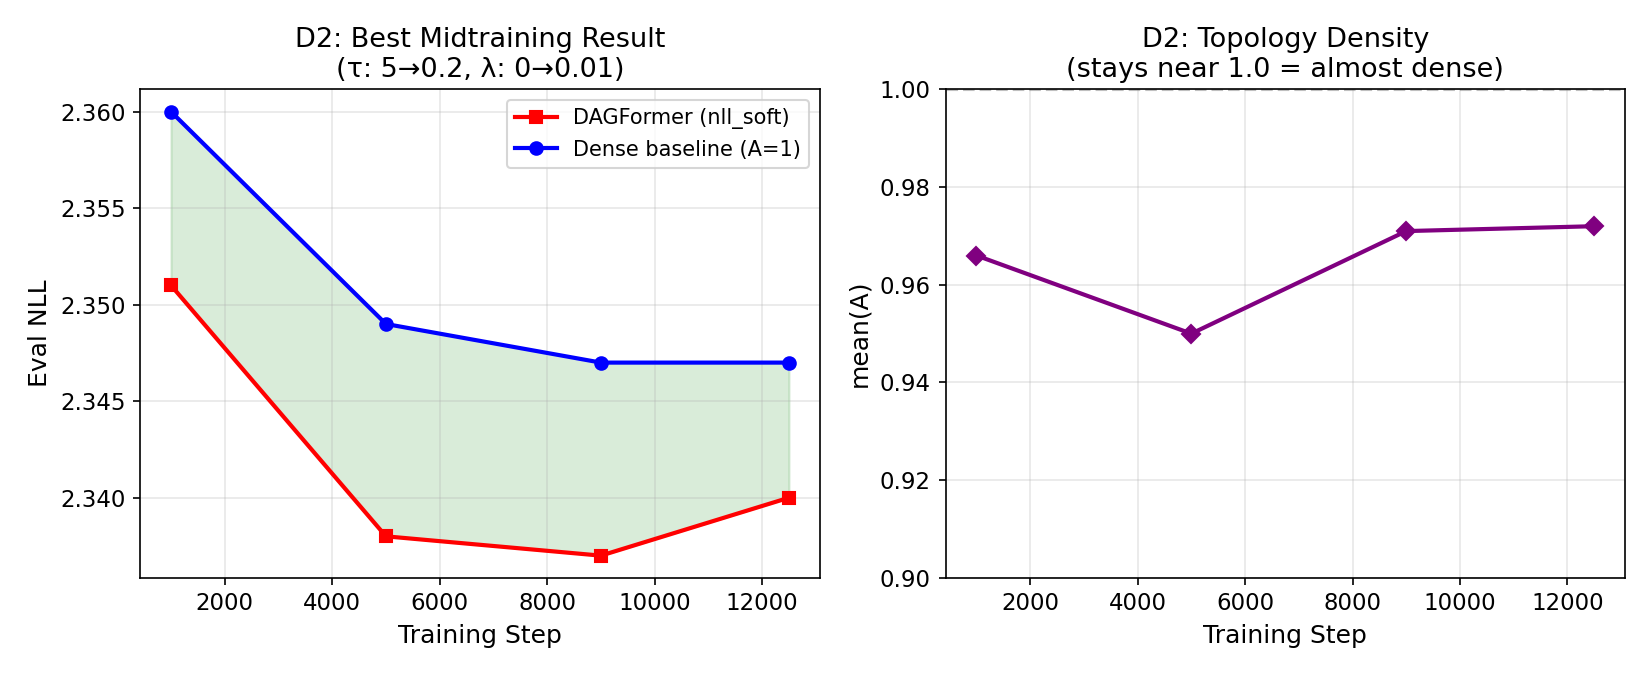
\includegraphics[width=0.88\textwidth]{figures/fig4_D2_trajectory.png}
\caption{D2 ($\tau$: $5\to0.2$, $\lambda$: $0\to0.01$) achieved $-0.007$ NLL vs baseline, but topology stayed near-dense (mean $\A \approx 0.97$) and \texttt{jaccard\_var}$=0$ throughout (no context-dependent routing). The improvement is statistically significant ($p < 10^{-6}$, $n=500$ paired $t$-test) but tiny and context-independent.}
\label{fig:d2}
\end{figure}

%───────────────────────────────────────────────────────────
\subsection{Summary: All Midtraining Experiments}

\begin{table}[H]
\centering
\small
\begin{tabular}{llllrrr}
\toprule
\textbf{Exp} & \textbf{OLMo LR} & \textbf{Pred LR} & \textbf{Strategy} & \textbf{NLL$-$Base} & \textbf{mean $\A$} & \textbf{Jaccard} \\
\midrule
P2-trial & 3e-5 & 1e-4 & Default           & $+0.001$ & 0.98 & 0 \\
P2a      & 3e-5 & 1e-2 & High pred LR      & $+0.228$ & 0.50 & 0 \\
P2b      & 5e-6 & 1e-3 & Low OLMo LR       & $\mathbf{-0.002}$ & 0.99 & 0 \\
P2c      & 1e-5 & 1e-3 & Med OLMo LR       & $+0.003$ & 0.99 & 0 \\
P2d      & 3e-5 & 1e-3 & Low $\tau$+init   & $+0.001$ & 0.99 & 0 \\
P2e      & 5e-6 & 1e-3 & +Sparsity         & $+0.008$ & 0.97 & 0 \\
P2f      & 5e-6 & 1e-3 & init\_logit=0      & $+0.475$ & 0.56 & 0 \\
D1       & 5e-6 & 1e-3 & $\A$ starts $\approx 0.5$ & $+0.186$ & 0.71 & 0 \\
D2       & 5e-6 & 1e-3 & $\tau$ anneal+$\lambda$ & $\mathbf{-0.007}$ & 0.97 & 0 \\
D6       & 5e-6 & 1e-3 & $\A$ starts $\approx 0$ & $+0.301$ & 0.56 & 0 \\
\bottomrule
\end{tabular}
\caption{All midtraining experiments on OLMo-1B. \texttt{Jaccard}=0 everywhere: the predictor produces identical topology for all inputs (no context-dependence).}
\label{tab:midtrain}
\end{table}

\subsection{Why Midtraining Failed}

Pretrained weights are optimized for dense connectivity. The loss landscape at $\A=\mathbf{1}$ is a \textbf{flat plateau} with near-zero gradient ($\sim\!4\!\times\!10^{-5}$), making gradient-based topology learning impossible. Joint training creates a chicken-and-egg problem: OLMo adapts to dense faster than the predictor can propose useful alternatives.

\textbf{Conclusion:} We need to train from scratch so that weights and topology co-evolve from random initialization.

%═══════════════════════════════════════════════════════════
\section{Pretraining from Scratch --- 300M OLMo-2}
%═══════════════════════════════════════════════════════════

We switched to pretraining a 300M OLMo-2 (12 layers $\times$ 16 heads, $\A \in \mathbb{R}^{192 \times 192}$) from random init. Dense baseline: 10K steps on Dolma v1.7, 5.24B tokens, \textbf{eval NLL = 3.609}, throughput 81K tok/s (4$\times$A40).

%───────────────────────────────────────────────────────────
\subsection{DAGFormer Variants (Batch 1: From Scratch)}

Three predictor types, all from random init with the same 5.24B token budget:

\begin{table}[H]
\centering
\small
\begin{tabular}{lllrrrr}
\toprule
\textbf{Variant} & \textbf{Predictor} & \textbf{tok/s} & \textbf{Steps} & \textbf{NLL (soft)} & \textbf{Own baseline} & \textbf{mean $\A$} \\
\midrule
Baseline   & None (dense)        & 81K  & 10000  & 3.609 & ---  & 1.0  \\
Static     & Learnable $UV^\top$  & 23K  & $\sim$4690 & $\sim$5.89 & $\sim$5.98 & 0.98 \\
Self-embed & Mean-pool embed      & 23K  & $\sim$4670 & $\sim$5.75 & $\sim$5.96 & \textbf{0.42} \\
Qwen       & Frozen Qwen-0.6B     & 14K  & $\sim$2920 & $\sim$6.15 & $\sim$6.28 & 0.41 \\
\bottomrule
\end{tabular}
\caption{From-scratch pretraining results. All DAGFormer variants see $\sim$3.5$\times$ fewer tokens in the same wall time due to per-head assembly overhead.}
\label{tab:pretrain}
\end{table}

\begin{figure}[H]
\centering
\begin{minipage}[t]{0.48\textwidth}
\centering
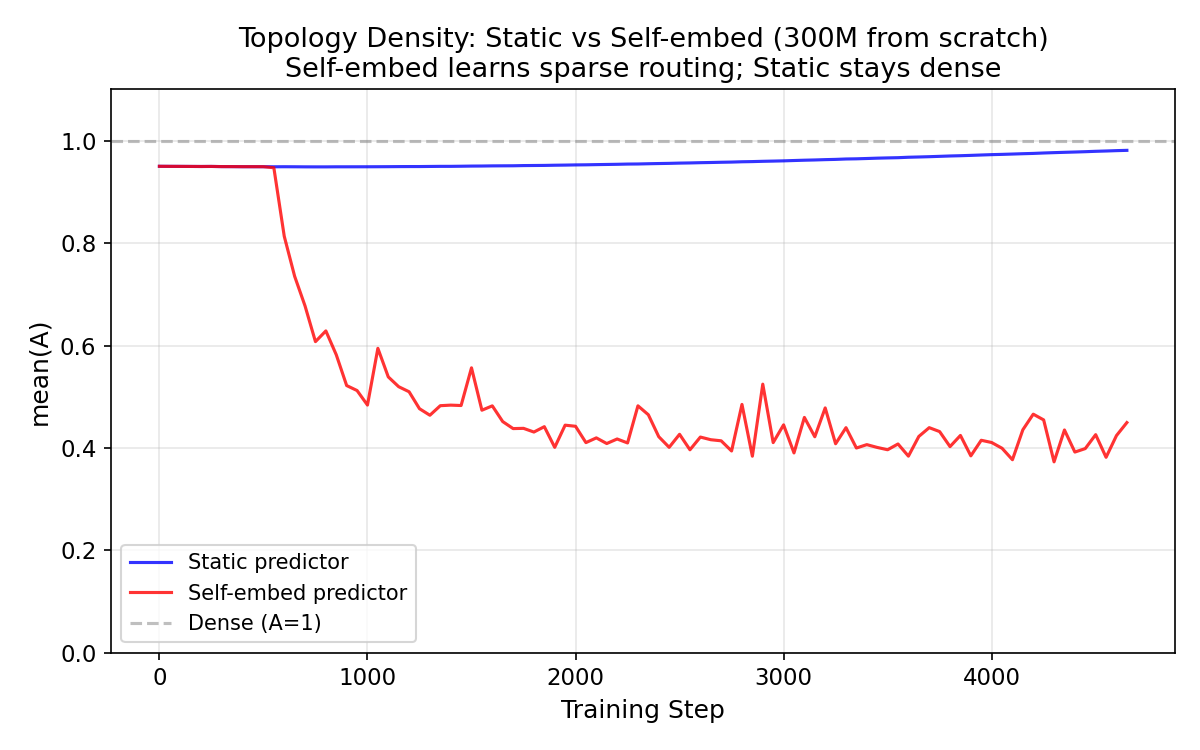
\includegraphics[width=\textwidth]{figures/fig6_meanA_static_vs_selfembed.png}
\captionof{figure}{Topology density over training. Self-embed rapidly learns sparse routing (mean $\A \to 0.42$), while Static stays dense. \textbf{First successful topology learning} across all experiments.}
\label{fig:meanA}
\end{minipage}\hfill
\begin{minipage}[t]{0.48\textwidth}
\centering
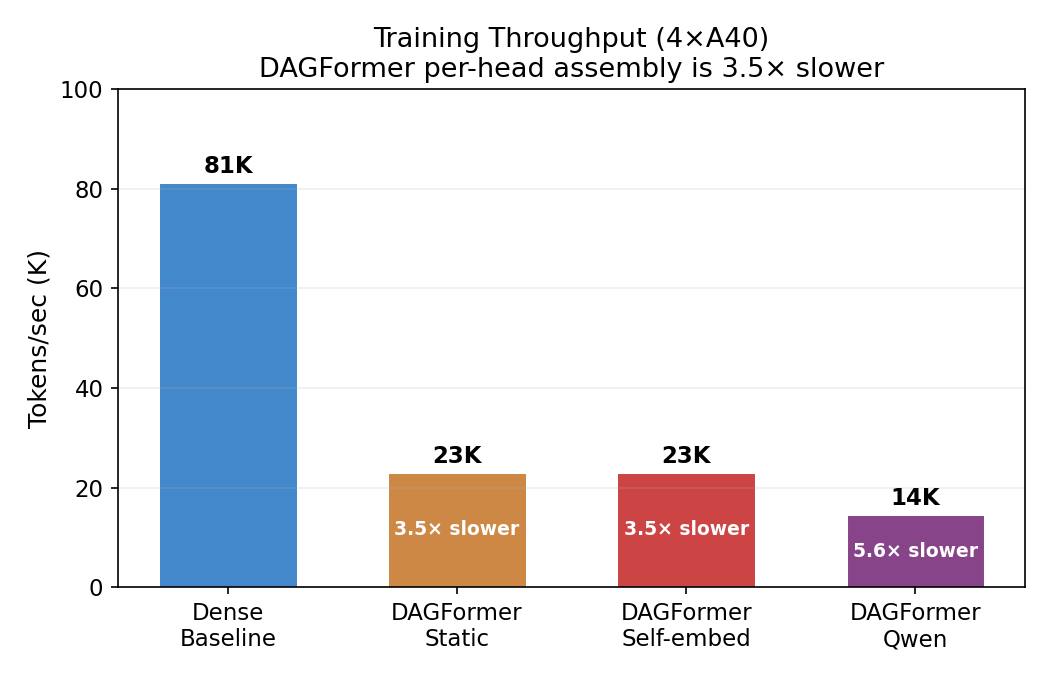
\includegraphics[width=\textwidth]{figures/fig7_throughput.png}
\captionof{figure}{Training throughput (4$\times$A40). Per-head input assembly makes DAGFormer 3.5$\times$ slower; Qwen adds another 1.6$\times$. Root cause of the NLL gap.}
\label{fig:throughput}
\end{minipage}
\end{figure}

\begin{figure}[H]
\centering
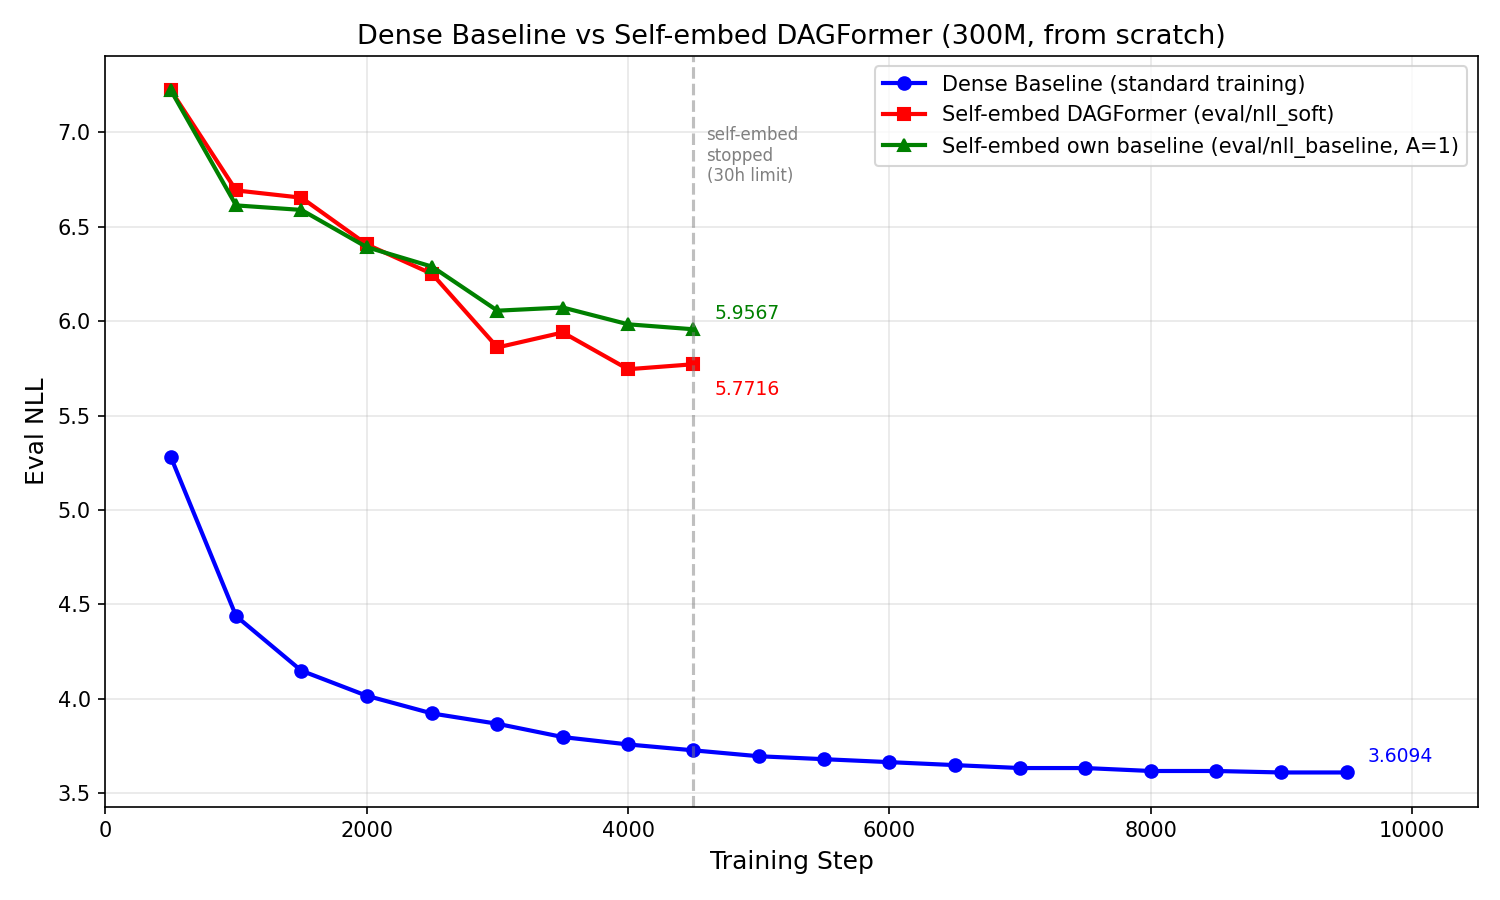
\includegraphics[width=0.82\textwidth]{nll_comparison_300m.png}
\caption{Eval NLL comparison. Blue: dense baseline. Red: self-embed DAGFormer (\texttt{eval/nll\_soft}). Green: self-embed's own dense forward ($\A=\mathbf{1}$). Key: red $<$ green after step 3000 --- learned topology helps the same undertrained model, but both are far behind the dense baseline due to throughput difference.}
\label{fig:nll_compare}
\end{figure}

\paragraph{Key findings.}
\begin{itemize}[nosep]
\item \textbf{Self-embed learns sparse topology} (mean $\A = 0.42$). First experiment where the predictor meaningfully deviates from dense.
\item \textbf{Learned topology helps}: soft NLL ($5.75$) $<$ own-baseline NLL ($5.96$), a 0.21 nat improvement on the same undertrained model.
\item \textbf{Static predictor fails}: mean $\A = 0.98$, predictor gradient $\sim 0$. Without input-dependent signal, the predictor cannot learn.
\item \textbf{3.5$\times$ throughput overhead is the bottleneck}: the model sees far fewer tokens, so the base model is severely undertrained.
\end{itemize}


%═══════════════════════════════════════════════════════════
\section{Current Experiments (In Progress)}
%═══════════════════════════════════════════════════════════

To address the throughput bottleneck, we are testing five new strategies.

\subsection{Addressing Throughput}

\paragraph{Staged training.} Load a fully-trained baseline checkpoint (10K steps, NLL=3.609), then switch to DAGFormer forward for 2,000 additional steps. The base model starts with good language modeling; only needs to adapt to routing. Predictor starts fresh.

\paragraph{Alternating training.} Train from scratch with a 9:1 ratio of standard (fast) to DAGFormer (slow) steps. Both update the base model; the predictor only updates on DAGFormer steps. Expected throughput $\approx$ 90\% of baseline.

\paragraph{Self-embed without detach.} Same as staged, but gradients from the predictor flow back into the embedding layer (\texttt{.detach()} removed). The embedding learns to produce representations useful for both language modeling and topology prediction.

\subsection{Improving Predictor Input}

The original self-embed applies mean pooling over raw token embeddings --- essentially bag-of-words, losing all positional and syntactic information.

\paragraph{Mini-encoder (independent).} Separate embedding table ($100\text{K} \times 256$) + 2-layer transformer encoder (dim=256, 4 heads). Learns its own contextual representation optimized for topology prediction. $\sim$41M parameters.

\paragraph{Context-embed (shared).} Reuses the LLM's embedding table, projects down ($1024 \to 256$), then applies a 2-layer transformer encoder. $\sim$16M parameters (no extra vocab cost). LLM embedding is detached.

\begin{table}[H]
\centering
\small
\begin{tabular}{clllr}
\toprule
\textbf{\#} & \textbf{Name} & \textbf{Strategy} & \textbf{Predictor Input} & \textbf{Steps} \\
\midrule
1 & Staged         & Baseline ckpt $\to$ DAGFormer    & Self-embed (mean pool)            & 2,000  \\
2 & Alternating    & 9:1 standard:DAGFormer           & Self-embed (mean pool)            & 10,000 \\
3 & No-detach      & Baseline ckpt + no detach        & Self-embed (unfrozen)             & 2,000  \\
4 & Mini-encoder   & Baseline ckpt                    & Independent 2L transformer        & 2,000  \\
5 & Context-embed  & Baseline ckpt                    & Shared embed + 2L transformer     & 2,000  \\
\bottomrule
\end{tabular}
\caption{Five new experiments currently running. Key axes: staged vs.\ alternating, detach vs.\ no-detach, bag-of-words vs.\ contextual input, independent vs.\ shared embedding.}
\label{tab:current}
\end{table}


%═══════════════════════════════════════════════════════════
\section{Discussion \& Next Steps}
%═══════════════════════════════════════════════════════════

\subsection{The Core Tension}

DAGFormer faces a fundamental speed--quality tradeoff. Per-head input assembly ($\text{input}_j = \text{base} + \sum_i \A[i,j] \cdot \text{head\_out}_i$) requires layer-sequential einsum operations, making it $\sim$3.5$\times$ slower than standard batched attention. More DAGFormer steps means better topology but fewer total tokens and a worse base model. Our current experiments explore different points on this tradeoff.

\subsection{Open Questions}

\begin{enumerate}[nosep]
\item \textbf{Does context-dependent topology matter?} Static failed, but may just need different optimization. If a fixed topology suffices, the predictor is unnecessary at inference.
\item \textbf{Can we amortize the overhead?} Sparse $\A$ (skip zero gates), fused kernels, or applying DAGFormer to only a subset of layers.
\item \textbf{What is the right predictor architecture?} Mean-pooled embeddings are too crude; a full Qwen encoder is too expensive. Mini-encoder and context-embed are middle ground --- is 2 transformer layers enough?
\item \textbf{Optimal model scale?} 300M may be too small (fewer redundant heads). Would 1B+ show clearer benefits?
\item \textbf{Distillation?} Train a dense teacher, distill into a DAGFormer student with sparse topology for inference efficiency.
\end{enumerate}

\subsection{Proposed Future Recipes}

\begin{table}[H]
\centering
\small
\begin{tabularx}{\textwidth}{lXX}
\toprule
\textbf{Recipe} & \textbf{Description} & \textbf{Rationale} \\
\midrule
Aggressive alternating & 50:1 or 100:1 standard:DAGFormer ratio & Near-baseline throughput; predictor gets minimal but possibly sufficient signal \\
Layer-subset DAGFormer & Apply $\A$ only to last 4 layers & Reduce overhead to $\sim$1.5$\times$; early layers may not need routing \\
Sparse $\A$ forward & Skip einsum for $\A[i,j] < 0.01$ & Exploit learned sparsity for speed (mean $\A = 0.42$ $\Rightarrow$ 58\% skippable) \\
Distillation & Dense teacher $\to$ sparse student & Decouple topology learning from language modeling \\
Curriculum & Short seq (256) first, then increase & Faster DAGFormer at small seq\_len \\
Scale up & 1B model from scratch & More heads = more redundancy = more room for topology \\
\bottomrule
\end{tabularx}
\caption{Proposed future recipes for team discussion.}
\label{tab:recipes}
\end{table}

\subsection{Summary}

We have established that: (1)~midtraining topology onto pretrained models does not work --- the loss landscape is flat at $\A=\mathbf{1}$; (2)~pretraining from scratch enables topology learning (self-embed achieves mean $\A=0.42$ with sparse routing that outperforms its own dense baseline); (3)~the main bottleneck is the 3.5$\times$ throughput overhead. Five strategies are currently under evaluation, and additional recipes are proposed above for team discussion.

\end{document}
